\chapter{Partitioning}
\label{chap:partitioning}

The ability to partition regions into {\em subregions} is a core
feature of Legion.  Many parallel programming systems have some notion
of a distributed collection---a collection of data that is broken up
into pieces and put in different places across a distributed machine.  In
Legion, the facilities for partitioning data are more expressive than most
ther programming systems in
several important ways.  First, partitioning can be done recursively
to arbitrary levels: regions can be partitioned into subregions, which
can themselves be partitioned further into additional
subregions, and
so on.  The partitioning hierarchy defines a tree, called the {\em
  region tree}, that is a useful abstraction of how data is organized
in a Legion application.  An important step in designing a Legion
application is deciding how data will be partitioned---i.e., deciding
what the region tree will look like.

A second distinguishing characteristic is that partitioning is done dynamically: The application can create and destroy region partitions at runtime.  Thus, Legion can naturally express methods where the organization of data needs to change during the computation, such as adaptive mesh refinement algorithms.  It is worth remembering, however, that partitioning can be an expensive operation, so it is important that it be used judiciously.  As long as the cost of the partitioning is amortized over lots of computation on the partition's subregions, no performance problems from partitioning will arise.

A third distinguishing characteristic is that partitions are themselves first-class objects in Legion.  A {\em partition} is a collection of subregions, and Legion
has many different built-in operations for creating useful partitions; presenting the
most common of these methods for partitioning data is the heart of this chapter.

Partitions do not need to be mathematical partitions, in fact
in Legion a partition can be {\em any} set of subsets of a region.
It is important to keep in mind that partitions only name subsets of data;
a partition does not allocate storage for the subregions or make copies of data.
This feature of partitions leads to some useful programming idioms.  For example, a program
can create a very large region, perhaps with billions of elements, and
then partition it and only materialize needed subregions, which is useful
in cases where there is a very large potential domain but only a relatively
small subset will actually be used.  It is also common to create a region
too large to fit in any physical memory, partition it into subregions that will
fit on each node, and then create physical instances only of the subregions.
The global name space is still useful (e.g., in neighbor computations for stencils)
even if the parent region is never physically allocated.

The subregions in a partition can overlap (share elements), in which
case we say the partition is {\em aliased}; otherwise the partition is
{\em disjoint}.  For example, aliased subregions can be useful in
describing stencil patterns, where the subblocks overlap by the width
of the stencil perations.  A {\em complete} partition is one in which
every element of the partitioned region is in at least one subregion
of the partition.  Partitions in Legion do not need to be complete; as an example,
it is often useful to name only the overlapping boundaries of blocks in stencils (the so-called {\em ghost regions}, which are a strict subset of the entire computational domain.

These idioms for using partitions are illustrated in the examples in the Legion repository.  In this tutorial we focus on illustrating the basic application of
the most commonly used Legion partitioning operators.

\section{Equal Partitions}
\label{sec:equal}

The simplest and most common case of partitioning is an {\em equal}
partition, where a region is automatically partitioned into subregions
of approximately equal size.  Figure~\ref{fig:equalpart} gives an
example of partitioning a region into four equal-size subregions.  The
number of subregions in the partition is given by an index space, with
one subregion created for each of the index space's points.  On line
17 of Figure~\ref{fig:equalpart} an index space with four points is
created from a 1D {\tt Rect} defined on line 16.  This set of {\em
  colors} (the term for the points in an index space
used for naming the subregions of a partition) is passed as an
argument to {\tt create\_equal\_partition} on line 18.  Note that the
partitioning operation is applied to the index space, not directly to
a logical region.  By partitioning the index space, the same
partitioning can be reused for multiple logical regions that share an
index space.  The {\tt get\_logical\_partition} call on line 19
returns the logical partition of the region defined by the index
partition.

Lines 25-28 illustrate an important Legion idiom where an index launch is performed
over the subregions of a partition.  Here the {\tt sum\_task} is applied to each
subregion of the {\tt lp} partition of the region {\tt lr}.   Note that {\tt IndexLauncher} created on line 25 uses the color space of the partition as its launch domain.  A region requirement for {\tt sum\_task} is added to the launcher on line 26.
We saw region requirements in Chapter~\ref{chap:regions} for launches of individual
tasks.  Region requirements for index launches have slightly different arguments:

\begin{itemize}
\item For an index launch the first argument is a logical partition. (For an individual task the first argument is a logical region.)

\item If the first argument is a logical partition, then the second argument is the identifier of a {\em projection functor} $f$. For index point $i$ in the launch space
  and logical partition $lp$,,
  the task is passed $f(lp,i)$ as its argument.   Projection function 0 is predefined to return the $i$th subregion for the $i$th point in the launch domain---i.e., the task will be applied to every subregion of $lp$, which is the most common case in practice. Users can write and register their own projection functors with the runtime
  system, much like task registration, for more complex patterns of selecting
  the arguemnts to index tasks from a region tree.

\item The rest of the fields are the same for both kinds of region requirements: the privilege for the region ({\tt READ\_ONLY} in this example), the coherence mode ({\tt EXCLUSIVE}), and the parent region ({\tt lr}) from which privileges are derived.
\end{itemize}
On line 27 the field {\tt FIELD\_A} is added to the region requirement.  The naming of the fields in a region requirment is separated from the region requirement's construction because any number of fields can be part of a region requirement; these are all the fields that the task will touch with the given permissions and coherence mode.

The execution of the launcher on line 28 runs {\tt sum\_task} on all the subregion sof {\tt lp}.  Instead of summing the entire region, the same {\tt sum\_task} is now used to sum all four subregions separately.


An equal partition is an example of a mathematical partition: an equal partition is always both disjoint (none of the subregions overlap) and complete (every element of the region is included in some subregion).

The runtime does not guarantee anything about equal partitions other than that the subreqions will be of approximately the same size.  At the time of this writing, for example, an equal partition of a multidimensional region will partition the region in just the first dimension.  If a specific kind of equal partition is desired other partitioning operators can be used.  For example, a blocked partition can be created with partition by restriction (see Section~\ref{sec:pbr}).




\begin{figure}
  {\small
   \lstinputlisting[linerange={15-49}]{Examples/Partitions/equal/equal.cc}
  }
  \caption{\legionbook{Partitions/equal/equal.cc}}
  \label{fig:equalpart}
\end{figure}


\section{Partition by Field}
\label{sec:pbf}

Equal partitioning leaves the choice of how to partition the elements of a region
up to the runtime system, requiring only that the sizes of subregions are
equal or nearly equal.  At the other extreme is {\em partition by field}, where
the application prescribes for each individual element of a region which subregion it should be assigned to.

The program in Figure~\ref{fig:pbf} illustrates partitioning by field.  This example is similar to the previous one,
but there is now an additional field {\tt FIELD\_PARTITION} that holds a coloring of the elements of the region.
The {\tt color\_launcher} on lines 23-26 invokes the {\tt color\_task} which assigns a color (a {\tt Point<1>} in this example; colors can also be multidimensional points) to each
element of the region.  In this case the assignment is a simple blocking, with each contiguous quarter of the elements assigned the same
color (lines 46-56; the function uses the number of colors as the divisor, which is 4 in this example), but the coloring could be any assignment of the color space to the elements of the field.  Note also that the
coloring is dynamically computed; programs can compute a coloring for a field and then partition the region accordingly.

The actual partitioning of the index space occurs on line 28.  The runtime call {\tt create\_partition\_by\_field} takes the current
context, the region, the parent region (or the same region if it has no parent, as in this case), and the field with the coloring.
On line 29 the partition of the index space is used to retrieve the logical partition.

The logic for launching the {\tt sum\_task} over the paritition on lines 31-35 is the same as in Figure~\ref{fig:equalpart}.

\begin{figure}
  {\small
   \lstinputlisting[linerange={17-74}]{"Examples/Partitions/partition_by_field/pbf.cc"}
  }
  \caption{\legionbook{Partitions/partition\_by\_field/pbf.cc}}
  \label{fig:pbf}
\end{figure}

\section{Partition by Restriction}
\label{sec:pbr}

\begin{figure}
  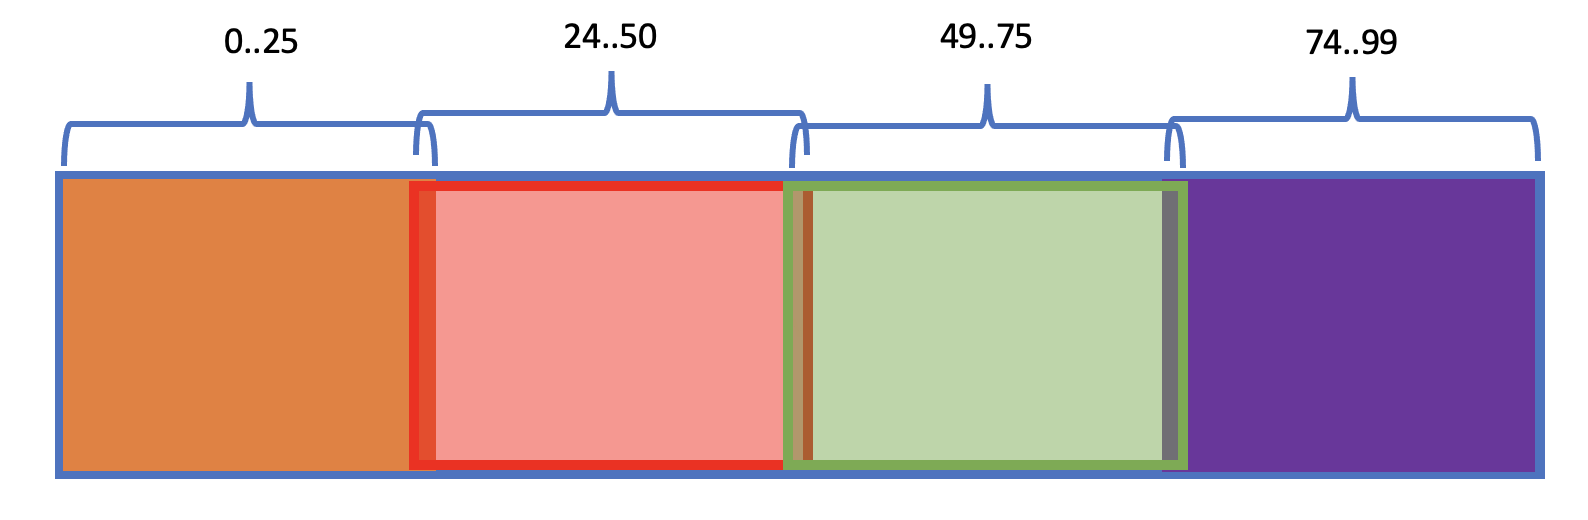
\includegraphics[height=1.5in]{figs/pbr.png}
  \caption{A blocked partition of a 1D region with ghost elements.}
  \label{fig:1dpbr}
\end{figure}

Another common partitioning idiom is to divide a region into blocks of the same size, a {\em blocked partitioning}.  For applications involving stencils, it can
also be useful for the blocks to include ``ghost cells'' adjacent to the block, essentially expanding the block in one or more dimensions.
Figure~\ref{fig:1dpbr} shows a 1D region partitioned into four subblocks, where each block includes one ghost element on each side.  For
a 1D region of 100 elements as shown in the figure, the result is four subblocks of size 26, 27, 27, and 26:  the two interior blocks have a ghost element on each side, while the first and last blocks have one ghost element each as the other element would be out of bounds of the region.

Figure~\ref{fig:pbr} gives code for computing the partitioning shown in Figure~\ref{fig:1dpbr}.  The essential differences from previous
  examples are on lines 21-27.  Starting with the {\tt create\_partition\_by\_restriction} call itself on line 27, we see that in addition to the
  usual context, index space, and color space this operation also takes a {\em transform} and an {\em extent}.  The extent $E$ is a ``generic''
  rectangle of the desired size---all subregions in the partition will have the shape of $E$.  The {\tt transform} $T$ is an
  $n \times m$ matrix, where $n$ is the number of dimensions of the color space and $m$ is the number of dimensions of the region.
  For a point $p$ in the color space, the points in the corresponding subregion are defined by the rectangle $Tp + E$.  That is $Tp$ defines
  an offset that is added to $E$ to name the points in the subregion associated with $p$.

  In this example, since the region and color space are both 1D, the transform is a 1x1 matrix, a single integer (lines 21-23); this transform
  says that subregions will start 25 elements apart (the {\tt blocksize}).  The extent defined on
  line 26 says that a subregion will extend one element to the left and 25 elements to the right of the 0-point of the subregion, so
  in general each subregion will have 27 elements.  Legion automatically clips any subregions that extend beyond the bounds of the region
  being partitioned, so for a color space of $\tt 0, 1, 2, 3$ the corresponding subregions will have elements $\tt 0..25, 24..50, 49..75, 74..99$.
  Note that unlike the other partitioning operations we have seen so far, the values of the color space are significant and affect the position
  of the subregion---for a region with an index space 0..99, it is necessary that the color space be $0..3$ and not some other set of four points.

\begin{figure}
  {\small
   \lstinputlisting[linerange={15-49}]{"Examples/Partitions/partition_by_restriction/pbr.cc"}
  }
  \caption{\legionbook{Partitions/partition\_by\_restriction/pbr.cc}}
  \label{fig:pbr}
\end{figure}


\section{Set-Based Partitions}
\label{sec:set}

Equal partitions, partitions by field and partitions by restriction are all examples of {\em independent} partitions, which are partitions that do
not depend on other partitions.  Legion also provides a number of {\em dependent} partitioning operators that take partitions as input and
produce partitions as output.  Dependent partitioning is used heavily in most Legion programs; it is not uncommon to see long chains of
partitioning operators to name complex subsets of the data that the program needs to manipulate. 

An {\em difference} partition takes two index space partitions and computes their set difference by color: A subspace of the difference partition
is the set difference of two subspaces, one from each of the two argument partitions, with the same color.  Thus, there is a subspace in the difference
partition for every color that the two argument partitions have in common.

Figure~\ref{fig:sets} gives an example that creates two partitions by restriction: a ``big'' partition that includes blocks of 26 elements spaced 25 elements apart (lines 22-28, similar to  the partition in Figure~\ref{fig:pbf} but with only one ghost element per subspace) and a ``small'' partition that is a disjoint partition of blocks of 25 elements spaced 25 elements apart (lines 22-24, 26, and 29). The region has 101 elements (line 6) to ensure that every subspace of the big partition actually has 26 elements (i.e., no elements are clipped for being out of bounds).  The difference partition subtracts the small partition from the big partition, so each subspace in the index partition names exactly the ghost element of the corresponding big subspace.  The result of the {\tt sum\_task} shows that there is exactly one element in each subregion of the difference partition.

Legion also provides {\tt create\_partition\_by\_union}, which
computes the set union of two partitions, and {\tt
  create\_partition\_by\_intersection}, which computes the set intersection
of two partitions.  These dependent
partitioning functions have the same signature as {\tt
  create\_partition\_by\_difference}.


\begin{figure}
  {\small
   \lstinputlisting[linerange={21-58}]{Examples/Partitions/sets/sets.cc}
  }
  \caption{\legionbook{Partitions/sets/sets.cc}}
  \label{fig:sets}
\end{figure}


\section{Image Partitions}
\label{sec:image}

\begin{figure}
  \centering
  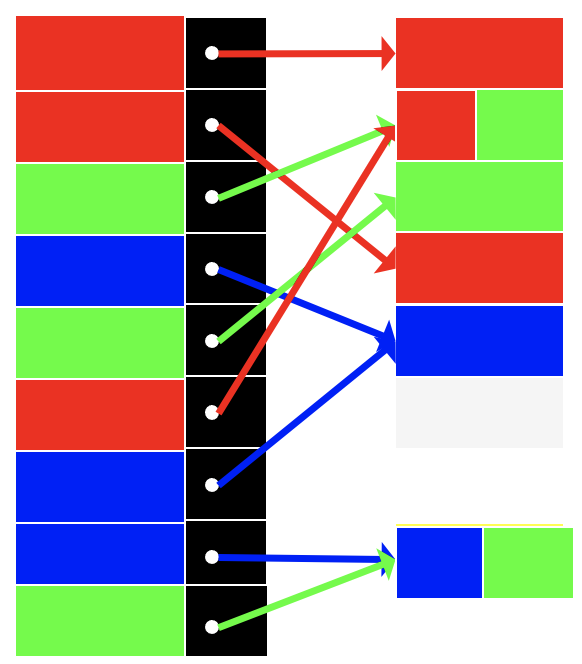
\includegraphics[height=2in]{figs/image.png}
  \caption{An image coloring.}
  \label{fig:eximage}
\end{figure}

  
Often we need to partition a region in a way compatible with an already computed partition of another region.
For example, consider a graph represented by a region of nodes and a region of edges. Assume we have chosen a partition of the nodes $\tt P_N[0],\ldots,P_N[k]$.
We will often want to partition the edges into subregions $\tt P_E[0],\ldots,P_E[k]$ such that the edges in $\tt P_E[i]$ all have source (or alternatively destination) nodes in $\tt P_N[i]$.  The {\em image} and {\em preimage} partitioning operators discussed in this section and the next provide mechanisms for using a pointer relationship between
two regions to induce a partitioning of one region given a partitioning of the other.

The example in Figure~\ref{fig:image} creates two regions.  The region {\tt lr\_src} (line 19) has a single field {\tt FIELD\_PTR} of type \verb+Point<1>+ (line 10).  Pointers
between regions are represented by points in the index space of the pointed-to region, which in this case is {\tt lr\_dst} (line 20).  The {\tt ptr\_task} (defined on lines 47-60 and called on lines 32-36) assigns pointers so that the $i$th element of {\tt lr\_src} points to the $i$th element of {\tt lr\_dst}.

The example creates an equal partition of {\tt lr\_src} on lines 29-30.  The {\tt create\_partition\_by\_image} ``transfers'' the partition of {\tt lr\_src} to the index space {\tt is}: if we think of the pointer field as a function from the source region to the destination index space and visualize the source partition as a coloring of the elements, then each pointer copies the color of its source element to the element of the destination.  An
example (unrelated to Figure~\ref{fig:image}) of taking the image of a pointer field under a partitioning of the source region is depicted in Figure~\ref{fig:eximage}.  In this abstract example, the coloring of the elements on the region on the left is copied via the pointer field to the elements of the index space or region on the right.  Because an element in the destination may have multiple pointers to it from the source, elements of the destination may have multiple colors, illustratedby the elements with two colors in Figure~\ref{fig:eximage}.  Thus, in general, the partition computed by {\tt create\_partition\_by\_image} may be aliased.  It may also be incomplete, as some elements of the destination region may have no pointers to them at all.  Because the pointer relationship is 1-1 between the source and destination regions
in the program in Figure~\ref{fig:image}, the partition of the destination in this case is both disjoint and complete.

The {\tt create\_partition\_by\_image} call on line 38 takes the current context, the index space to be partitioned, the source region partition, the source region, the identity of the pointer field in the source region, and the color space of the partition to be computed.  The result is an {\tt IndexPartition} of the destination index space.

The rest of the program (lines 41-45) sums the value field of the destination partition's subregions (which as in other examples has the same value 1 for every element).  Since the 1-1 pointer relationship copies the coloring exactly from source to destination and the source was an equal partition, the sums printed for each subregion are the same.

\begin{figure}
  {\small
    \lstinputlisting[linerange={17-76}]{Examples/Partitions/image/image.cc}
  }
  \caption{\legionbook{Partitions/image/image.cc}}
  \label{fig:image}
\end{figure}

\section{Pre-Image Partitions}
\label{sec:preimage}


\begin{figure}
  \centering
  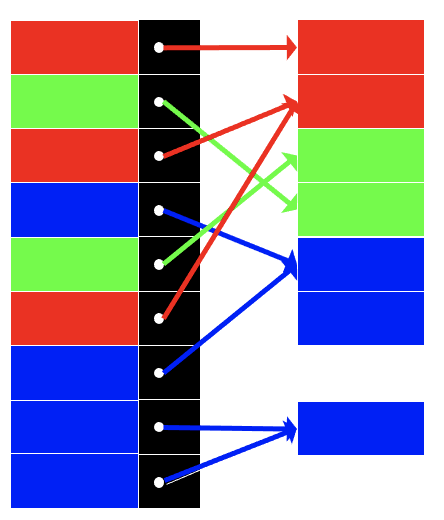
\includegraphics[height=2in]{figs/preimage.png}
  \caption{An preimage coloring.}
  \label{fig:expreimage}
\end{figure}

Where an image partition transfers a partitioning from a pointer's source region to its destination, a pre-image transfers a partitioning of the destination to the source.  Viewing
the pointer field as a function from source to destination, this operation is a preimage computation of that function.

The program in Figure~\ref{fig:preimage} gives an example.  As before there is a source region and a destination index space.  (Note that the source must be a region because
we need a pointer field, and only regions have fields.)  The source region has both the pointer field and the value field (lines 8-11), because we will be summing the subregions computed
by the preimage operation, which are subregions of the source region.  We do not need any fields in the destination region in this simple example, so its field space is empty (line 13).

Line 32 creates an equal partition {\tt ip\_dst} of the index space {\tt is} of the destination region.  The call to {\tt create\_partition\_by\_preimage} on line 35 transfers this partitioning backwards across the pointer field {\tt FIELD\_PTR} to the index space of the source region.  The call takes the current context, the partition of the destination index space, the source region, the source region's parent (or the source region itself if it has no parent, as in this example), the name of the pointer field in the source region, and the color space for the computed partition.

Figure~\ref{fig:expreimage} gives an abstract example of a preimage computation.  Here the pre-existing partition is on the right, and the color of each element is copied backwards through the pointer field to derive a coloring (a partitioning) of the source index space.  Note that because a pointer has a single source, a preimage is always guaranteed to be a disjoint partitioning of the source (but the partition may be incomplete---not every element of the source necessarily has a pointer into the destination).

Returning to the program in Figure~\ref{fig:preimage}, lines 38-43 sum the elements of the value field of each of the subregions of the source.  Again in this example the $i$th element of the source points to the $i$th element of the destination (lines 24-27 and 45-58), so the preimage operation replicates the equal partition of the destination in the source index space.  Since the value field is initialized to 1 (lines 21-22), the sums count the number of elements of each source subregion, which are all equal.


\begin{figure}
  {\small
   \lstinputlisting[linerange={17-74}]{"Examples/Partitions/pre_image/preimage.cc"}
  }
  \caption{\legionbook{Partitions/pre\_image/preimage.cc}}
  \label{fig:preimage}
\end{figure}

